% Created by tikzDevice version 0.10.1 on 2018-02-17 16:56:30
% !TEX encoding = UTF-8 Unicode
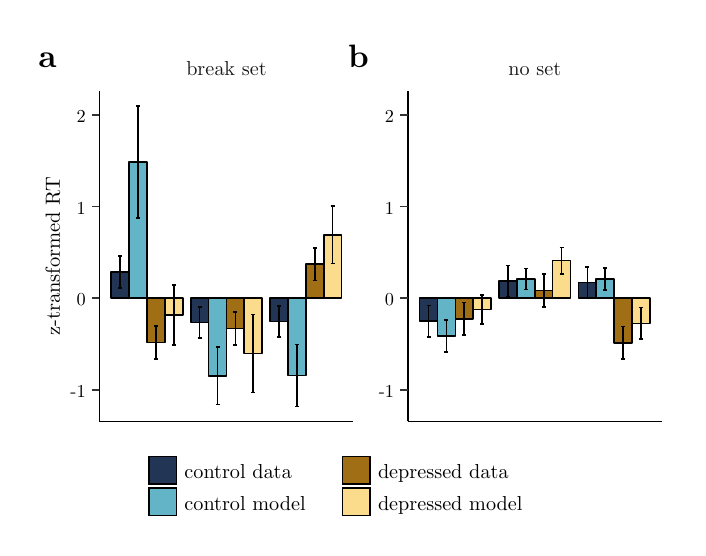
\begin{tikzpicture}[x=1pt,y=1pt]
\definecolor{fillColor}{RGB}{255,255,255}
\path[use as bounding box,fill=fillColor,fill opacity=0.00] (0,0) rectangle (234.88,180.67);
\begin{scope}
\path[clip] (  0.00, 30.11) rectangle (234.64,180.67);
\definecolor{drawColor}{RGB}{255,255,255}
\definecolor{fillColor}{RGB}{255,255,255}

\path[draw=drawColor,line width= 0.6pt,line join=round,line cap=round,fill=fillColor] (  0.00, 30.11) rectangle (234.64,180.67);
\end{scope}
\begin{scope}
\path[clip] ( 25.92, 38.36) rectangle (117.73,157.69);
\definecolor{fillColor}{RGB}{255,255,255}

\path[fill=fillColor] ( 25.92, 38.36) rectangle (117.73,157.69);
\definecolor{drawColor}{RGB}{0,0,0}
\definecolor{fillColor}{RGB}{250,220,140}

\path[draw=drawColor,line width= 0.6pt,line join=round,fill=fillColor] ( 49.59, 76.75) rectangle ( 56.05, 82.88);
\definecolor{fillColor}{RGB}{160,110,20}

\path[draw=drawColor,line width= 0.6pt,line join=round,fill=fillColor] ( 43.14, 66.90) rectangle ( 49.59, 82.88);
\definecolor{fillColor}{RGB}{100,180,200}

\path[draw=drawColor,line width= 0.6pt,line join=round,fill=fillColor] ( 36.68, 82.88) rectangle ( 43.14,132.02);
\definecolor{fillColor}{RGB}{35,53,85}

\path[draw=drawColor,line width= 0.6pt,line join=round,fill=fillColor] ( 30.22, 82.88) rectangle ( 36.68, 92.40);
\definecolor{fillColor}{RGB}{250,220,140}

\path[draw=drawColor,line width= 0.6pt,line join=round,fill=fillColor] ( 78.28, 62.90) rectangle ( 84.74, 82.88);
\definecolor{fillColor}{RGB}{160,110,20}

\path[draw=drawColor,line width= 0.6pt,line join=round,fill=fillColor] ( 71.83, 71.94) rectangle ( 78.28, 82.88);
\definecolor{fillColor}{RGB}{100,180,200}

\path[draw=drawColor,line width= 0.6pt,line join=round,fill=fillColor] ( 65.37, 54.89) rectangle ( 71.83, 82.88);
\definecolor{fillColor}{RGB}{35,53,85}

\path[draw=drawColor,line width= 0.6pt,line join=round,fill=fillColor] ( 58.92, 74.16) rectangle ( 65.37, 82.88);
\definecolor{fillColor}{RGB}{250,220,140}

\path[draw=drawColor,line width= 0.6pt,line join=round,fill=fillColor] (106.97, 82.88) rectangle (113.43,105.82);
\definecolor{fillColor}{RGB}{160,110,20}

\path[draw=drawColor,line width= 0.6pt,line join=round,fill=fillColor] (100.52, 82.88) rectangle (106.97, 95.18);
\definecolor{fillColor}{RGB}{100,180,200}

\path[draw=drawColor,line width= 0.6pt,line join=round,fill=fillColor] ( 94.06, 54.99) rectangle (100.52, 82.88);
\definecolor{fillColor}{RGB}{35,53,85}

\path[draw=drawColor,line width= 0.6pt,line join=round,fill=fillColor] ( 87.61, 74.53) rectangle ( 94.06, 82.88);

\path[draw=drawColor,line width= 0.6pt,line join=round] ( 52.10, 87.58) --
	( 53.54, 87.58);

\path[draw=drawColor,line width= 0.6pt,line join=round] ( 52.82, 87.58) --
	( 52.82, 65.92);

\path[draw=drawColor,line width= 0.6pt,line join=round] ( 52.10, 65.92) --
	( 53.54, 65.92);

\path[draw=drawColor,line width= 0.6pt,line join=round] ( 45.65, 72.78) --
	( 47.08, 72.78);

\path[draw=drawColor,line width= 0.6pt,line join=round] ( 46.36, 72.78) --
	( 46.36, 61.01);

\path[draw=drawColor,line width= 0.6pt,line join=round] ( 45.65, 61.01) --
	( 47.08, 61.01);

\path[draw=drawColor,line width= 0.6pt,line join=round] ( 39.19,152.26) --
	( 40.63,152.26);

\path[draw=drawColor,line width= 0.6pt,line join=round] ( 39.91,152.26) --
	( 39.91,111.78);

\path[draw=drawColor,line width= 0.6pt,line join=round] ( 39.19,111.78) --
	( 40.63,111.78);

\path[draw=drawColor,line width= 0.6pt,line join=round] ( 32.74, 98.21) --
	( 34.17, 98.21);

\path[draw=drawColor,line width= 0.6pt,line join=round] ( 33.45, 98.21) --
	( 33.45, 86.59);

\path[draw=drawColor,line width= 0.6pt,line join=round] ( 32.74, 86.59) --
	( 34.17, 86.59);

\path[draw=drawColor,line width= 0.6pt,line join=round] ( 80.79, 76.98) --
	( 82.23, 76.98);

\path[draw=drawColor,line width= 0.6pt,line join=round] ( 81.51, 76.98) --
	( 81.51, 48.81);

\path[draw=drawColor,line width= 0.6pt,line join=round] ( 80.79, 48.81) --
	( 82.23, 48.81);

\path[draw=drawColor,line width= 0.6pt,line join=round] ( 74.34, 77.81) --
	( 75.77, 77.81);

\path[draw=drawColor,line width= 0.6pt,line join=round] ( 75.05, 77.81) --
	( 75.05, 66.07);

\path[draw=drawColor,line width= 0.6pt,line join=round] ( 74.34, 66.07) --
	( 75.77, 66.07);

\path[draw=drawColor,line width= 0.6pt,line join=round] ( 67.88, 65.24) --
	( 69.32, 65.24);

\path[draw=drawColor,line width= 0.6pt,line join=round] ( 68.60, 65.24) --
	( 68.60, 44.55);

\path[draw=drawColor,line width= 0.6pt,line join=round] ( 67.88, 44.55) --
	( 69.32, 44.55);

\path[draw=drawColor,line width= 0.6pt,line join=round] ( 61.43, 79.82) --
	( 62.86, 79.82);

\path[draw=drawColor,line width= 0.6pt,line join=round] ( 62.14, 79.82) --
	( 62.14, 68.50);

\path[draw=drawColor,line width= 0.6pt,line join=round] ( 61.43, 68.50) --
	( 62.86, 68.50);

\path[draw=drawColor,line width= 0.6pt,line join=round] (109.48,116.19) --
	(110.92,116.19);

\path[draw=drawColor,line width= 0.6pt,line join=round] (110.20,116.19) --
	(110.20, 95.45);

\path[draw=drawColor,line width= 0.6pt,line join=round] (109.48, 95.45) --
	(110.92, 95.45);

\path[draw=drawColor,line width= 0.6pt,line join=round] (103.03,101.07) --
	(104.46,101.07);

\path[draw=drawColor,line width= 0.6pt,line join=round] (103.74,101.07) --
	(103.74, 89.30);

\path[draw=drawColor,line width= 0.6pt,line join=round] (103.03, 89.30) --
	(104.46, 89.30);

\path[draw=drawColor,line width= 0.6pt,line join=round] ( 96.57, 66.20) --
	( 98.01, 66.20);

\path[draw=drawColor,line width= 0.6pt,line join=round] ( 97.29, 66.20) --
	( 97.29, 43.79);

\path[draw=drawColor,line width= 0.6pt,line join=round] ( 96.57, 43.79) --
	( 98.01, 43.79);

\path[draw=drawColor,line width= 0.6pt,line join=round] ( 90.12, 80.20) --
	( 91.55, 80.20);

\path[draw=drawColor,line width= 0.6pt,line join=round] ( 90.83, 80.20) --
	( 90.83, 68.87);

\path[draw=drawColor,line width= 0.6pt,line join=round] ( 90.12, 68.87) --
	( 91.55, 68.87);
\end{scope}
\begin{scope}
\path[clip] (137.33, 38.36) rectangle (229.14,157.69);
\definecolor{fillColor}{RGB}{255,255,255}

\path[fill=fillColor] (137.33, 38.36) rectangle (229.14,157.69);
\definecolor{drawColor}{RGB}{0,0,0}
\definecolor{fillColor}{RGB}{250,220,140}

\path[draw=drawColor,line width= 0.6pt,line join=round,fill=fillColor] (161.00, 78.86) rectangle (167.46, 82.88);
\definecolor{fillColor}{RGB}{160,110,20}

\path[draw=drawColor,line width= 0.6pt,line join=round,fill=fillColor] (154.55, 75.51) rectangle (161.00, 82.88);
\definecolor{fillColor}{RGB}{100,180,200}

\path[draw=drawColor,line width= 0.6pt,line join=round,fill=fillColor] (148.09, 69.23) rectangle (154.55, 82.88);
\definecolor{fillColor}{RGB}{35,53,85}

\path[draw=drawColor,line width= 0.6pt,line join=round,fill=fillColor] (141.64, 74.65) rectangle (148.09, 82.88);
\definecolor{fillColor}{RGB}{250,220,140}

\path[draw=drawColor,line width= 0.6pt,line join=round,fill=fillColor] (189.69, 82.88) rectangle (196.15, 96.52);
\definecolor{fillColor}{RGB}{160,110,20}

\path[draw=drawColor,line width= 0.6pt,line join=round,fill=fillColor] (183.24, 82.88) rectangle (189.69, 85.67);
\definecolor{fillColor}{RGB}{100,180,200}

\path[draw=drawColor,line width= 0.6pt,line join=round,fill=fillColor] (176.78, 82.88) rectangle (183.24, 89.89);
\definecolor{fillColor}{RGB}{35,53,85}

\path[draw=drawColor,line width= 0.6pt,line join=round,fill=fillColor] (170.33, 82.88) rectangle (176.78, 89.13);
\definecolor{fillColor}{RGB}{250,220,140}

\path[draw=drawColor,line width= 0.6pt,line join=round,fill=fillColor] (218.38, 73.82) rectangle (224.84, 82.88);
\definecolor{fillColor}{RGB}{160,110,20}

\path[draw=drawColor,line width= 0.6pt,line join=round,fill=fillColor] (211.93, 66.78) rectangle (218.38, 82.88);
\definecolor{fillColor}{RGB}{100,180,200}

\path[draw=drawColor,line width= 0.6pt,line join=round,fill=fillColor] (205.47, 82.88) rectangle (211.93, 89.77);
\definecolor{fillColor}{RGB}{35,53,85}

\path[draw=drawColor,line width= 0.6pt,line join=round,fill=fillColor] (199.02, 82.88) rectangle (205.47, 88.64);

\path[draw=drawColor,line width= 0.6pt,line join=round] (163.51, 84.17) --
	(164.95, 84.17);

\path[draw=drawColor,line width= 0.6pt,line join=round] (164.23, 84.17) --
	(164.23, 73.54);

\path[draw=drawColor,line width= 0.6pt,line join=round] (163.51, 73.54) --
	(164.95, 73.54);

\path[draw=drawColor,line width= 0.6pt,line join=round] (157.06, 81.38) --
	(158.49, 81.38);

\path[draw=drawColor,line width= 0.6pt,line join=round] (157.78, 81.38) --
	(157.78, 69.64);

\path[draw=drawColor,line width= 0.6pt,line join=round] (157.06, 69.64) --
	(158.49, 69.64);

\path[draw=drawColor,line width= 0.6pt,line join=round] (150.60, 75.00) --
	(152.04, 75.00);

\path[draw=drawColor,line width= 0.6pt,line join=round] (151.32, 75.00) --
	(151.32, 63.46);

\path[draw=drawColor,line width= 0.6pt,line join=round] (150.60, 63.46) --
	(152.04, 63.46);

\path[draw=drawColor,line width= 0.6pt,line join=round] (144.15, 80.33) --
	(145.58, 80.33);

\path[draw=drawColor,line width= 0.6pt,line join=round] (144.87, 80.33) --
	(144.87, 68.97);

\path[draw=drawColor,line width= 0.6pt,line join=round] (144.15, 68.97) --
	(145.58, 68.97);

\path[draw=drawColor,line width= 0.6pt,line join=round] (192.20,101.29) --
	(193.64,101.29);

\path[draw=drawColor,line width= 0.6pt,line join=round] (192.92,101.29) --
	(192.92, 91.76);

\path[draw=drawColor,line width= 0.6pt,line join=round] (192.20, 91.76) --
	(193.64, 91.76);

\path[draw=drawColor,line width= 0.6pt,line join=round] (185.75, 91.55) --
	(187.18, 91.55);

\path[draw=drawColor,line width= 0.6pt,line join=round] (186.47, 91.55) --
	(186.47, 79.78);

\path[draw=drawColor,line width= 0.6pt,line join=round] (185.75, 79.78) --
	(187.18, 79.78);

\path[draw=drawColor,line width= 0.6pt,line join=round] (179.29, 93.67) --
	(180.73, 93.67);

\path[draw=drawColor,line width= 0.6pt,line join=round] (180.01, 93.67) --
	(180.01, 86.11);

\path[draw=drawColor,line width= 0.6pt,line join=round] (179.29, 86.11) --
	(180.73, 86.11);

\path[draw=drawColor,line width= 0.6pt,line join=round] (172.84, 94.79) --
	(174.27, 94.79);

\path[draw=drawColor,line width= 0.6pt,line join=round] (173.56, 94.79) --
	(173.56, 83.47);

\path[draw=drawColor,line width= 0.6pt,line join=round] (172.84, 83.47) --
	(174.27, 83.47);

\path[draw=drawColor,line width= 0.6pt,line join=round] (220.89, 79.56) --
	(222.33, 79.56);

\path[draw=drawColor,line width= 0.6pt,line join=round] (221.61, 79.56) --
	(221.61, 68.07);

\path[draw=drawColor,line width= 0.6pt,line join=round] (220.89, 68.07) --
	(222.33, 68.07);

\path[draw=drawColor,line width= 0.6pt,line join=round] (214.44, 72.65) --
	(215.87, 72.65);

\path[draw=drawColor,line width= 0.6pt,line join=round] (215.16, 72.65) --
	(215.16, 60.92);

\path[draw=drawColor,line width= 0.6pt,line join=round] (214.44, 60.92) --
	(215.87, 60.92);

\path[draw=drawColor,line width= 0.6pt,line join=round] (207.98, 93.76) --
	(209.42, 93.76);

\path[draw=drawColor,line width= 0.6pt,line join=round] (208.70, 93.76) --
	(208.70, 85.78);

\path[draw=drawColor,line width= 0.6pt,line join=round] (207.98, 85.78) --
	(209.42, 85.78);

\path[draw=drawColor,line width= 0.6pt,line join=round] (201.53, 94.30) --
	(202.96, 94.30);

\path[draw=drawColor,line width= 0.6pt,line join=round] (202.25, 94.30) --
	(202.25, 82.98);

\path[draw=drawColor,line width= 0.6pt,line join=round] (201.53, 82.98) --
	(202.96, 82.98);
\end{scope}
\begin{scope}
\path[clip] ( 25.92,157.69) rectangle (117.73,175.17);
\definecolor{drawColor}{RGB}{255,255,255}
\definecolor{fillColor}{RGB}{255,255,255}

\path[draw=drawColor,line width= 1.1pt,line join=round,line cap=round,fill=fillColor] ( 25.92,157.69) rectangle (117.73,175.17);
\definecolor{drawColor}{gray}{0.10}

\node[text=drawColor,anchor=base,inner sep=0pt, outer sep=0pt, scale=  0.73] at ( 71.83,163.40) {break set};
\end{scope}
\begin{scope}
\path[clip] (137.33,157.69) rectangle (229.14,175.17);
\definecolor{drawColor}{RGB}{255,255,255}
\definecolor{fillColor}{RGB}{255,255,255}

\path[draw=drawColor,line width= 1.1pt,line join=round,line cap=round,fill=fillColor] (137.33,157.69) rectangle (229.14,175.17);
\definecolor{drawColor}{gray}{0.10}

\node[text=drawColor,anchor=base,inner sep=0pt, outer sep=0pt, scale=  0.73] at (183.24,163.40) {no set};
\end{scope}
\begin{scope}
\path[clip] (  0.00,  0.00) rectangle (234.88,180.67);
\definecolor{drawColor}{RGB}{0,0,0}

\path[draw=drawColor,line width= 0.6pt,line join=round] ( 25.92, 38.36) --
	(117.73, 38.36);
\end{scope}
\begin{scope}
\path[clip] (  0.00,  0.00) rectangle (234.88,180.67);
\definecolor{drawColor}{RGB}{0,0,0}

\path[draw=drawColor,line width= 0.6pt,line join=round] (137.33, 38.36) --
	(229.14, 38.36);
\end{scope}
\begin{scope}
\path[clip] (  0.00,  0.00) rectangle (234.88,180.67);
\definecolor{drawColor}{RGB}{0,0,0}

\path[draw=drawColor,line width= 0.6pt,line join=round] (137.33, 38.36) --
	(137.33,157.69);
\end{scope}
\begin{scope}
\path[clip] (  0.00,  0.00) rectangle (234.88,180.67);
\definecolor{drawColor}{RGB}{0,0,0}

\node[text=drawColor,anchor=base east,inner sep=0pt, outer sep=0pt, scale=  0.66] at (132.38, 47.00) {-1};

\node[text=drawColor,anchor=base east,inner sep=0pt, outer sep=0pt, scale=  0.66] at (132.38, 80.16) {0};

\node[text=drawColor,anchor=base east,inner sep=0pt, outer sep=0pt, scale=  0.66] at (132.38,113.31) {1};

\node[text=drawColor,anchor=base east,inner sep=0pt, outer sep=0pt, scale=  0.66] at (132.38,146.46) {2};
\end{scope}
\begin{scope}
\path[clip] (  0.00,  0.00) rectangle (234.88,180.67);
\definecolor{drawColor}{gray}{0.20}

\path[draw=drawColor,line width= 0.6pt,line join=round] (134.58, 49.73) --
	(137.33, 49.73);

\path[draw=drawColor,line width= 0.6pt,line join=round] (134.58, 82.88) --
	(137.33, 82.88);

\path[draw=drawColor,line width= 0.6pt,line join=round] (134.58,116.04) --
	(137.33,116.04);

\path[draw=drawColor,line width= 0.6pt,line join=round] (134.58,149.19) --
	(137.33,149.19);
\end{scope}
\begin{scope}
\path[clip] (  0.00,  0.00) rectangle (234.88,180.67);
\definecolor{drawColor}{RGB}{0,0,0}

\path[draw=drawColor,line width= 0.6pt,line join=round] ( 25.92, 38.36) --
	( 25.92,157.69);
\end{scope}
\begin{scope}
\path[clip] (  0.00,  0.00) rectangle (234.88,180.67);
\definecolor{drawColor}{RGB}{0,0,0}

\node[text=drawColor,anchor=base east,inner sep=0pt, outer sep=0pt, scale=  0.66] at ( 20.97, 47.00) {-1};

\node[text=drawColor,anchor=base east,inner sep=0pt, outer sep=0pt, scale=  0.66] at ( 20.97, 80.16) {0};

\node[text=drawColor,anchor=base east,inner sep=0pt, outer sep=0pt, scale=  0.66] at ( 20.97,113.31) {1};

\node[text=drawColor,anchor=base east,inner sep=0pt, outer sep=0pt, scale=  0.66] at ( 20.97,146.46) {2};
\end{scope}
\begin{scope}
\path[clip] (  0.00,  0.00) rectangle (234.88,180.67);
\definecolor{drawColor}{gray}{0.20}

\path[draw=drawColor,line width= 0.6pt,line join=round] ( 23.17, 49.73) --
	( 25.92, 49.73);

\path[draw=drawColor,line width= 0.6pt,line join=round] ( 23.17, 82.88) --
	( 25.92, 82.88);

\path[draw=drawColor,line width= 0.6pt,line join=round] ( 23.17,116.04) --
	( 25.92,116.04);

\path[draw=drawColor,line width= 0.6pt,line join=round] ( 23.17,149.19) --
	( 25.92,149.19);
\end{scope}
\begin{scope}
\path[clip] (  0.00,  0.00) rectangle (234.88,180.67);
\definecolor{drawColor}{RGB}{0,0,0}

\node[text=drawColor,rotate= 90.00,anchor=base,inner sep=0pt, outer sep=0pt, scale=  0.74] at ( 11.64, 98.03) {z-transformed RT};
\end{scope}
\begin{scope}
\path[clip] (  0.00,  0.00) rectangle (234.88,180.67);
\definecolor{drawColor}{RGB}{0,0,0}

\node[text=drawColor,anchor=base west,inner sep=0pt, outer sep=0pt, scale=  1.17] at (  3.83,166.18) {\bfseries a};

\node[text=drawColor,anchor=base west,inner sep=0pt, outer sep=0pt, scale=  1.17] at (115.83,166.18) {\bfseries b};
\end{scope}
\begin{scope}
\path[clip] (  0.00,  0.00) rectangle (234.88,180.67);
\definecolor{fillColor}{RGB}{255,255,255}

\path[fill=fillColor] ( 33.07, -2.02) rectangle (201.57, 32.13);
\end{scope}
\begin{scope}
\path[clip] (  0.00,  0.00) rectangle (234.88,180.67);
\definecolor{drawColor}{RGB}{0,0,0}
\definecolor{fillColor}{RGB}{35,53,85}

\path[draw=drawColor,line width= 0.6pt,line cap=round,fill=fillColor] ( 43.81, 15.77) rectangle ( 53.77, 25.73);
\end{scope}
\begin{scope}
\path[clip] (  0.00,  0.00) rectangle (234.88,180.67);
\definecolor{drawColor}{RGB}{0,0,0}
\definecolor{fillColor}{RGB}{100,180,200}

\path[draw=drawColor,line width= 0.6pt,line cap=round,fill=fillColor] ( 43.81,  4.39) rectangle ( 53.77, 14.34);
\end{scope}
\begin{scope}
\path[clip] (  0.00,  0.00) rectangle (234.88,180.67);
\definecolor{drawColor}{RGB}{0,0,0}
\definecolor{fillColor}{RGB}{160,110,20}

\path[draw=drawColor,line width= 0.6pt,line cap=round,fill=fillColor] (113.75, 15.77) rectangle (123.71, 25.73);
\end{scope}
\begin{scope}
\path[clip] (  0.00,  0.00) rectangle (234.88,180.67);
\definecolor{drawColor}{RGB}{0,0,0}
\definecolor{fillColor}{RGB}{250,220,140}

\path[draw=drawColor,line width= 0.6pt,line cap=round,fill=fillColor] (113.75,  4.39) rectangle (123.71, 14.34);
\end{scope}
\begin{scope}
\path[clip] (  0.00,  0.00) rectangle (234.88,180.67);
\definecolor{drawColor}{RGB}{0,0,0}

\node[text=drawColor,anchor=base west,inner sep=0pt, outer sep=0pt, scale=  0.73] at ( 56.65, 17.72) {control data};
\end{scope}
\begin{scope}
\path[clip] (  0.00,  0.00) rectangle (234.88,180.67);
\definecolor{drawColor}{RGB}{0,0,0}

\node[text=drawColor,anchor=base west,inner sep=0pt, outer sep=0pt, scale=  0.73] at ( 56.65,  6.34) {control model};
\end{scope}
\begin{scope}
\path[clip] (  0.00,  0.00) rectangle (234.88,180.67);
\definecolor{drawColor}{RGB}{0,0,0}

\node[text=drawColor,anchor=base west,inner sep=0pt, outer sep=0pt, scale=  0.73] at (126.59, 17.72) {depressed data};
\end{scope}
\begin{scope}
\path[clip] (  0.00,  0.00) rectangle (234.88,180.67);
\definecolor{drawColor}{RGB}{0,0,0}

\node[text=drawColor,anchor=base west,inner sep=0pt, outer sep=0pt, scale=  0.73] at (126.59,  6.34) {depressed model};
\end{scope}
\end{tikzpicture}
